\section{What the exact theorem can be used for}
\label{sec:applications}

\subsection{A denominator budget for several matrices}

The aggregate conclusion is particularly natural when an arithmetic argument
charges a \emph{sum} of local denominator lengths.

\begin{corollary}[Simultaneous determinantal specialization]
\label{cor:matrices}
Let \(M_i(\mathbf T)\) be finitely many square matrices of bounded integral
power series over a finite extension \(E/\Q_p\). Suppose there are possibly
different points \(\mathbf x_i\), with every coordinate of valuation at
least \(\rho>0\), at which
\[
 \det M_i(\mathbf x_i)\ne0,\qquad
 \sum_i v(\det M_i(\mathbf x_i))\le B.
\]
At a common torsion tuple with every coordinate order between \(p^{h_0}\)
and \(p^{H_0}\), all matrices are nonsingular and
\[
                   \sum_i v(\det M_i(\boldsymbol\zeta-\mathbf1))\le B.
\]
If \(E'\) contains their specialized entries and \(e(E'/\Q_p)\) is its
ramification index, then
\[
 \sum_i \frac{\length_{\mathcal O_{E'}}
        \operatorname{coker}M_i(\boldsymbol\zeta-\mathbf1)}
               {e(E'/\Q_p)}
 \le B.
\]
\end{corollary}

\begin{proof}
Take \(F_i=\det M_i\) in Corollary~\ref{cor:aggregate}. The determinants
are bounded integral power series and satisfy the separate witness
hypothesis. Nonsingularity follows from the finite valuation bound.
Over a discrete valuation ring, Smith normal form gives
\(\length\operatorname{coker}M_i=v_{\pi_{E'}}(\det M_i)\).
The normalization is \(v_{\pi_{E'}}=e(E'/\Q_p)v\), proving the last
formula.
\end{proof}

For a rectangular matrix with \(r\) rows, choose an \(r\)-column minor
nonzero at its witness and apply the same argument to these chosen
determinants. The selected minor ensures full row rank. Its image is
contained in the image of the whole matrix, so the torsion cokernel of
the latter has no greater length. The same aggregate bound therefore
holds. This is a proved matrix statement; identifying a particular
Selmer module with such a cokernel is an additional arithmetic theorem.

This use matches part of the bookkeeping in the RH proof: denominator
losses are added after taking logarithms. It does not match every caller
of the original selector. Where each separate Selmer group must satisfy
its own prescribed threshold, the aggregate result is insufficient.
Proposition~\ref{prop:individual-obstruction} makes that limitation
unavoidable under the uniform assumptions considered here.

\subsection{Finite search and what the constants mean}

For \(s\) variables, the theorem specifies a finite set on which at least
one satisfactory specialization exists:
\[
 \left(\bigcup_{h=h_0}^{H_0}(U_h-1)\right)^s.
\]
The number of available scalar points is
\(p^{H_0}-p^{h_0-1}\). The grid therefore grows exponentially with \(s\)
and with \(H_0\); dimension independence of the \emph{order bound} does
not mean a dimension-independent search cost.

For explicit algebraic coefficients, one can enumerate cyclotomic
extensions and perform exact arithmetic to test candidates. For
arbitrary \(\C_p\) coefficients, this is an existence theorem:
it does not supply an effective encoding or a decidable equality test for
all possible coefficients. The power-series proof supplies a finite tail
cutoff, but that cutoff can be very large.

For \(p=3,h_0=2,B=1\), the exact theorem gives \(H_0=47\).
This means that one may choose some order \(3^h\) with \(2\le h\le47\).
It does not mean that the root has order \(47\), nor that order \(3^{47}\)
is necessary. The explicit bound is a uniform conservative guarantee.

\begin{table}[htbp]
\centering
\begin{tabular}{rrrr}
\toprule
$\delta$ & Prior $H$ & Refined $H_+$ & Exact $H_0$\\
\midrule
$1/2$ & 17 & 12 & 47\\
$1/10$ & 88 & 48 & 47\\
$1/100$ & 2,233 & 448 & 47\\
$1/1000$ & 69,026 & 4,448 & 47\\
\bottomrule
\end{tabular}

\caption{Safe upper bounds for the shell exponent at \(p=3,h_0=2,B=1\).
The prior and refined tolerance bounds allow error \(\delta\);
the exact bound allows error zero. These are sufficient bounds, not
lower bounds on the true optimal order.}
\label{tab:bounds}
\end{table}

\begin{figure}[htbp]
\centering
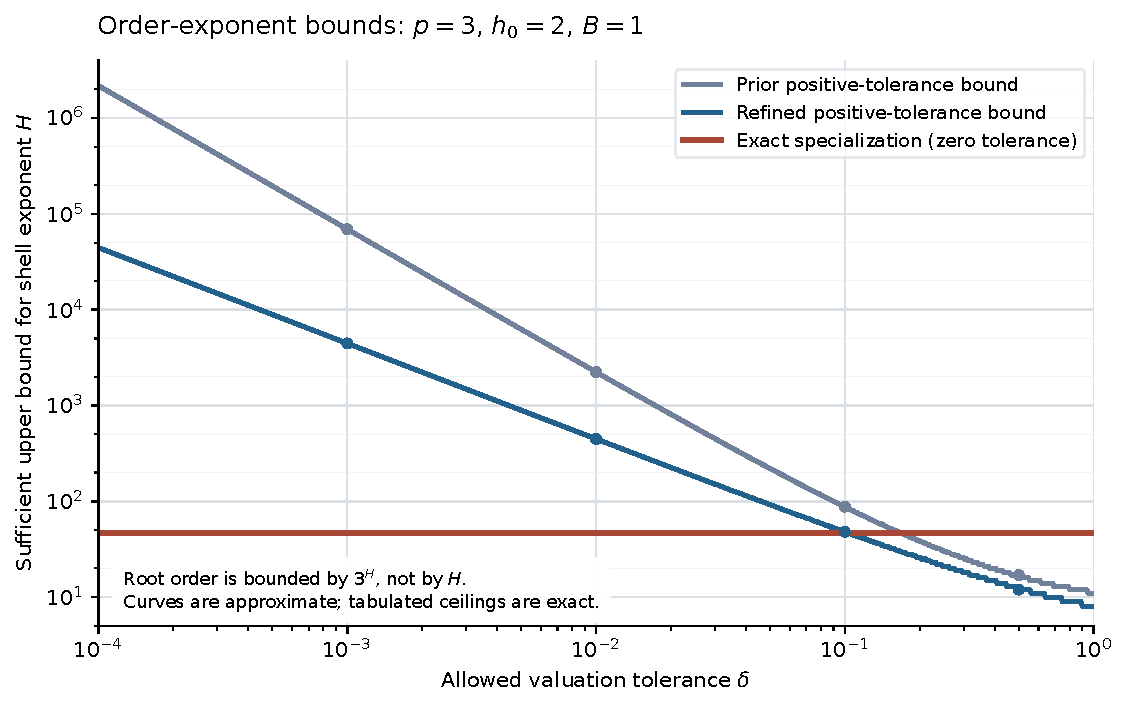
\includegraphics[width=0.92\linewidth]{figures/order_bounds.pdf}
\caption{Comparison of sufficient shell-exponent bounds for one function.
The plotted curves visualize the displayed formulas; the accompanying
table is computed with exact rational and integer-root arithmetic.
No empirical \(p\)-adic or prime-distribution data are used.}
\label{fig:bounds}
\end{figure}

\subsection{Twists and nonvanishing: a precise conditional use}

Suppose a particular arithmetic problem provides bounded integral
interpolation functions \(F_i(\mathbf T)\) whose values at torsion
parameters equal normalized special values or determinants, up to
explicit nonzero factors. Suppose it also provides nonzero witness values
with a total valuation budget \(B\). The theorem then selects a common
finite-order parameter at which all those interpolated values are nonzero
and their total valuation is at most \(B\). The first-powers construction
in Section~\ref{sec:exact-torsion} handles a finite list of powers of the
same parameter. If every first \(m\) power must be nontrivial, choose
\(p^{h_0}>m\).

This statement is useful only once the interpolation formula, integrality,
and witnesses are established. It is not a proof of nonvanishing when
the functions themselves are identically zero, when their coefficients
are unbounded, or when the chosen parameter space is not the allowed
arithmetic family. A bound on character order also does not bound the
norm of its conductor: the latter depends on where the character
ramifies and on the global realization of the local parameters.

There is substantial prior work on this subject. Kriz--Nordentoft
prove exact finite-group maximum-modulus principles and simultaneous
nonvanishing applications for horizontal \(p\)-adic \(L\)-functions
\cite{kn}. The exact comparison itself is therefore not a new general
phenomenon. Serban studies near-zero formal torsion loci, with
function-dependent thresholds under appropriate coefficient hypotheses
\cite{serban}. Schefer uses nearest-root arguments and cyclotomic distance
sums in quantitative torsion equidistribution; its bounds involve degree
and a polynomial-dependent separation constant \cite{schefer}.

The distinctive statement established here is the explicit order interval
depending only on a \emph{positive-radius Gauss budget}, uniformly in degree,
coefficient field, and number of coordinates. We did not locate this
particular bound in those primary sources. This targeted comparison is
not a proof of historical priority, and the theorem should not be
advertised as settling a previously named nonvanishing conjecture.

\subsection{Further restrictions that cannot be dropped}

The comparison radius must be positive. For \(F(T)=T\),
\(\G_0(F)=0\), while every nontrivial \(p\)-power root of unity has
\(v(F(\zeta-1))>0\). Thus an exact comparison with the coefficient
infimum at radius zero is false.

The coefficients must be bounded below in valuation. The series
\(\log(1+T)=\sum_{n\ge1}(-1)^{n+1}T^n/n\) converges on the open
unit disc and vanishes at every \(p\)-power torsion point shifted by
\(-1\), but its coefficients have unbounded negative valuations.
It is outside the theorem's hypotheses.

Finally, the theorem selects an order in an interval, not a prescribed
single shell. The integral polynomial \(\Phi_{p^H}(1+T)\) vanishes on
the entire primitive \(p^H\)-shell while its positive-radius Gauss
valuation is at most one. No universal assertion that the uppermost
shell itself works can hold under these hypotheses.

